%\only<presentation>{

%\lstset{language=C++, basicstyle=\ttfamily, 
%  keywordstyle=\color{red}\bfseries, tabsize=4, stringstyle=\ttfamily,
%  commentstyle=\it, extendedchars=true, escapeinside={/*@}{@*/}}

%\lstset{language=C++, basicstyle=\scriptsize\ttfamily,
%  stringstyle=\ttfamily, commentstyle=\it, extendedchars=true,
%  numbers=left, numberstyle=\tiny, stepnumber=2, numbersep=5pt,
%  breakatwhitespace=true, breaklines=true}
%\definecolor{darkgray}{gray}{0.4}
%\lstset{keywordstyle=\color{violet},
%        commentstyle=\color{darkgray},
%        stringstyle=\color{orange},
%        emph={bool,int,unsigned,char,true,false,void}, emphstyle=\color{blue},
%        emph={[2]\#include,\#define,\#ifdef,\#endif}, emphstyle={[2]\color{violet}},
%        }
%}
%\only<article>{
%\lstset{language=C++, basicstyle=\small, 
%  keywordstyle=\bfseries, tabsize=4, stringstyle=\ttfamily,
%  commentstyle=\it, extendedchars=true, escapeinside={/*@}{@*/}}

%\lstset{language=C++, basicstyle=\small\ttfamily,
%  stringstyle=\ttfamily, commentstyle=\it, extendedchars=true,
%  numbers=left, numberstyle=\tiny, stepnumber=2, numbersep=5pt,
%  breakatwhitespace=true, breaklines=true}
%\definecolor{darkgray}{gray}{0.4}
%\lstset{keywordstyle=\color{violet},
%        commentstyle=\color{darkgray},
%        stringstyle=\color{orange},
%        emph={bool,int,unsigned,char,true,false,void}, emphstyle=\color{blue},
%        emph={[2]\#include,\#define,\#ifdef,\#endif}, emphstyle={[2]\color{violet}},
%        }
%        }

\section{Parallel PDELab}
\subsection{Introduction}

\subsubsection{Why Parallel Computing?}

\begin{frame}
\frametitle<presentation>{Why Parallel Computing?}

\begin{itemize}
\item The speed of individual computer cores is not increasing 
essentially since some years
\item The number of cores is increasing. Dual-cores are the rule, 
up to 12-core processors are available.
\item Several multi-core processors can be used on one mainboard (e.g. four 12-core processors)
\item Computer cluster with several multi-core multi-processor servers are affordable even for small companies
\item High-performance computer have up to 294912 cores (JUGENE).
\end{itemize}

\end{frame}

%-----------------------------------------------------------------------------

\subsubsection{Architectures of Parallel Computers}

\begin{frame}
\frametitle<presentation>{Architectures of Parallel Computers}
\begin{itemize}
\item Shared-memory computing: all cores have access to the whole memory
\begin{itemize}
\item Uniform memory access architecture (UMA): access to every memory location from every processor takes the
same amount of time (multi-core CPUs)
\item Non-uniform memory access architecture (NUMA): memory is associated with processors but address space is 
global. Local memory can be accessed faster than memory attached
to other processors (multi-processor servers)
\end{itemize}
\item Message passing architecture (MP): each processor can only access local memory, information is exchanged
between processors with messages send over a network (computer clusters, super computer)
\end{itemize}
\end{frame}


\begin{frame}
\frametitle{Comparison of Architectures by Example}
\begin{itemize}
\item Given vectors $x,y\in\mathbb{R}^N$, compute scalar product $s =
  \sum_{i=0}^{N-1} x_i y_i$:
\begin{itemize}
\item[(1)] Subdivide index set into $P$ pieces. 
\item[(2)] Compute $s_p=\sum_{i=pN/P}^{(p+1)N/P-1} x_i y_i$ in
  parallel.
\item[(3)] Compute $s = \sum_{i=0}^{P-1} s_i$.
\end{itemize}
\item \textit{Uniform memory access architecture}: Store vectors as in
  sequential program:
\begin{center}
  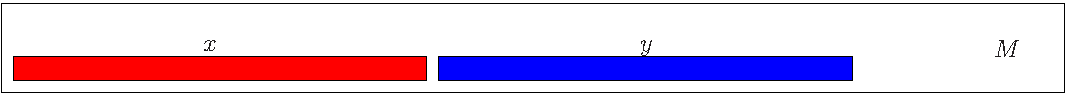
\includegraphics[width=0.9\textwidth]{EPS/umalayout}
\end{center}
\item \textit{Nonuniform memory access architecture}: Distribute
  data to the local memories:
\begin{center}
  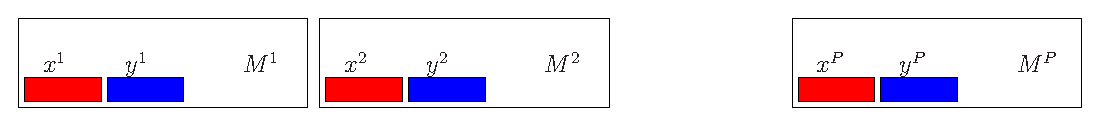
\includegraphics[width=0.9\textwidth]{EPS/numalayout}
\end{center}
\item \textit{Private memory architecture}: Same as for NUMA! 
\item Distributing data structures is hard and not automatic in
  general.
\item Parallelisation effort for NUMA and MP is almost the same.
\end{itemize}
\end{frame}


\subsubsection{Message Passing}
\begin{frame}
\frametitle<presentation>{Message Passing}

\begin{itemize}
\item Users view: Copy (contiguous) memory block from one address space to the
  other.
\item Message is subdivided into individual packets.
\item Network is packet-switched. 
\item A packet consists of an envelope and
  the data:
\begin{center}
  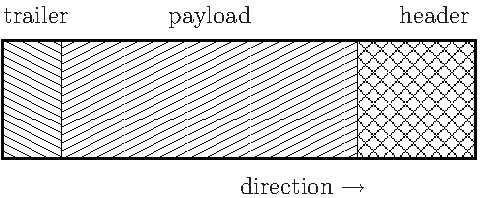
\includegraphics[width=0.49\textwidth]{EPS/paket}
\end{center}
\item Header: Destination, size and kind of data.
\item Payload: Size ranges from some bytes to kilobytes.
\item Trailer: E.g. checksum for error detection.
\end{itemize}
\end{frame}

%----------------------------------------------------------------------------------------
\begin{frame}
\frametitle{The Message Passing Interface (MPI)}

\begin{itemize}
\item Portable Library with functions for message exchange between processes
\item Developed 1993-94 by a international board
\item Available on nearly all computer platforms
\item Free Implementations also for LINUX Clusters: {\bf MPICH}\footnote{\href{http://www-unix.mcs.anl.gov/mpi/mpich}{{\tiny http://www-unix.mcs.anl.gov/mpi/mpich}}}
 and {\bf OpenMPI}\footnote{\href{http://www.open-mpi.org/}{{\tiny http://www.open-mpi.org/}}} (former {\bf LAM})
\item Properties of MPI:
\begin{itemize}
\item library with C-, C++ and Fortran bindings (no language extension)
\item large variety of point-to-point communication functions
\item global communication
\item data conversion for heterogeneous systems
\item subset formation and topologies possible
\end{itemize}

\end{itemize}

\begin{small}\textit{Remark:} There is a special MPICH version for shared-memory machines using memory copy operations instead of slower mesage passing algorithms.
OpenMPI can even distinguish between processes which share the same address space and
processes on remote machines and use either memory copy or message passing.
\end{small}
\end{frame}

\subsubsection{Strong Scalability Example}
\begin{frame}
\frametitle<presentation>{Strong Scalability of 3D Parallel Computation}
\begin{center}
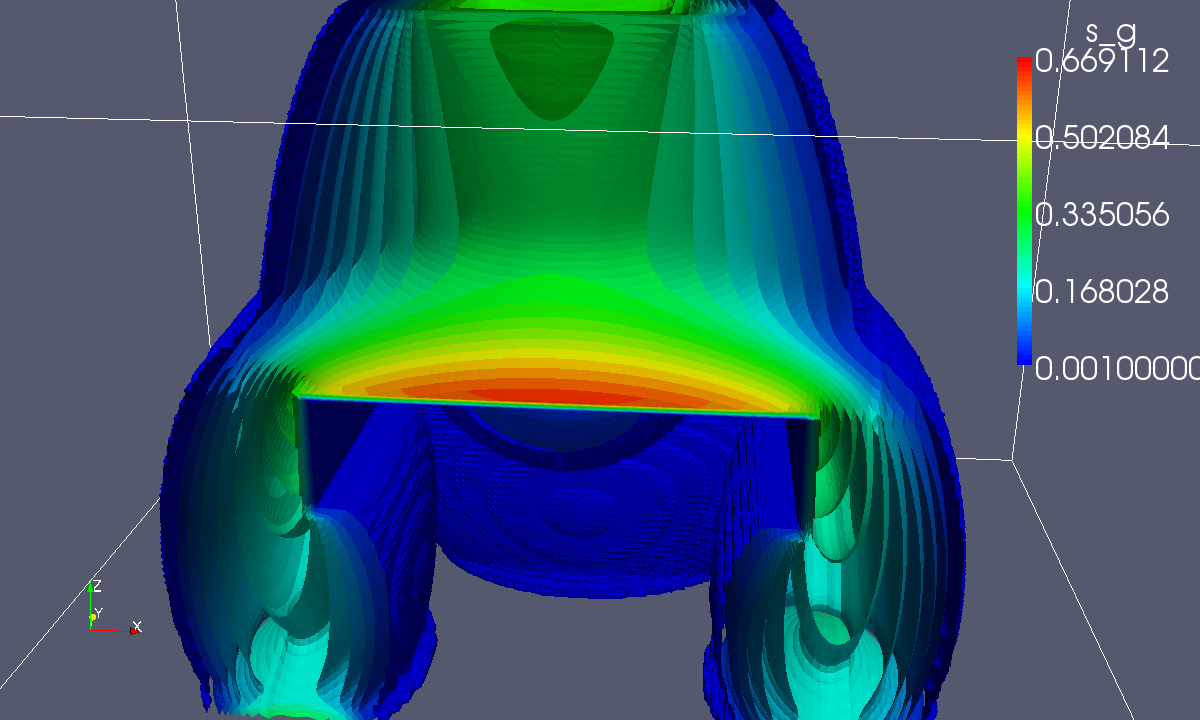
\includegraphics[width=0.9\textwidth]{EPS/dnapl-3d-het-iso}\\
3D DNAPL Infiltration
\end{center}
\end{frame}


\begin{frame}
\frametitle<presentation>{Strong Scalability of 3D Parallel Computation}
Simulation of a DNAPL infiltration with a coarse lense on a grid with  $160 \times 160 \times 96$
unknowns on a server with 4$\times$12  AMD Magny Cours, 2.1 GHz, 12$\times$0.5MB L2, 12MB
L3 processors.

Computation time for one time step with BiCGStab + AMG preconditioner:

\begin{center}
\begin{tabular}{r|rrr|rr|rr}
\hline
P  & \#IT(max) & $T_{it}$ & S & $T_{asm}$ & S & $T_{total}$ & S \\
\hline
 1  &  6.5 & 4.60 &      - &  43.7 &      - & 713.8 &    - \\
 4  &  10  & 1.85 &   2.5 &  17.5 &   2.5 & 295.9 & 2.4 \\
 8  &  9    & 0.63 &   7.3 &    8.4 &   5.2 & 127.1 & 5.6 \\
16 &  9.5 & 0.40 & 11.5 &    4.1 & 10.7 &   73.1 & 9.8 \\
32 &  15  & 0.27 & 17.0 &    1.9 & 23.0 &   43.5 & 16.4 \\ 
\hline
\end{tabular}
\end{center} 

Comparison with T3E from 1999

\begin{center}
\begin{tabular}{r|rrrr}
\hline
Machine  & Cells & Time steps & Newton steps & $T_{total}$ \\
\hline
256 T3E        & 2621440 &  50 & 264 & 14719\\
16 Cores AMD & 2457600 & 50 & 231 & 2500\\ 
\hline
\end{tabular}
\end{center} 
\end{frame}


\subsection{Domain Decomposition}
\begin{frame}
  \frametitle<presentation>{Domain Decomposition}

  \begin{itemize}
  \item partition a problem by splitting the domain it into small subdomains
  \item each part is solved by a different processor
  \item goes back to an idea of H.A. Schwarz who in 1890 presented a method to prove the existence of
        solutions of the Laplace equation on ``complicated'' domains.
  \item Different variants:
    \begin{itemize}
    \item overlapping domain decomposition
    \item non-overlapping domain decomposition
    \end{itemize}
  \end{itemize}
  
  \begin{center}
    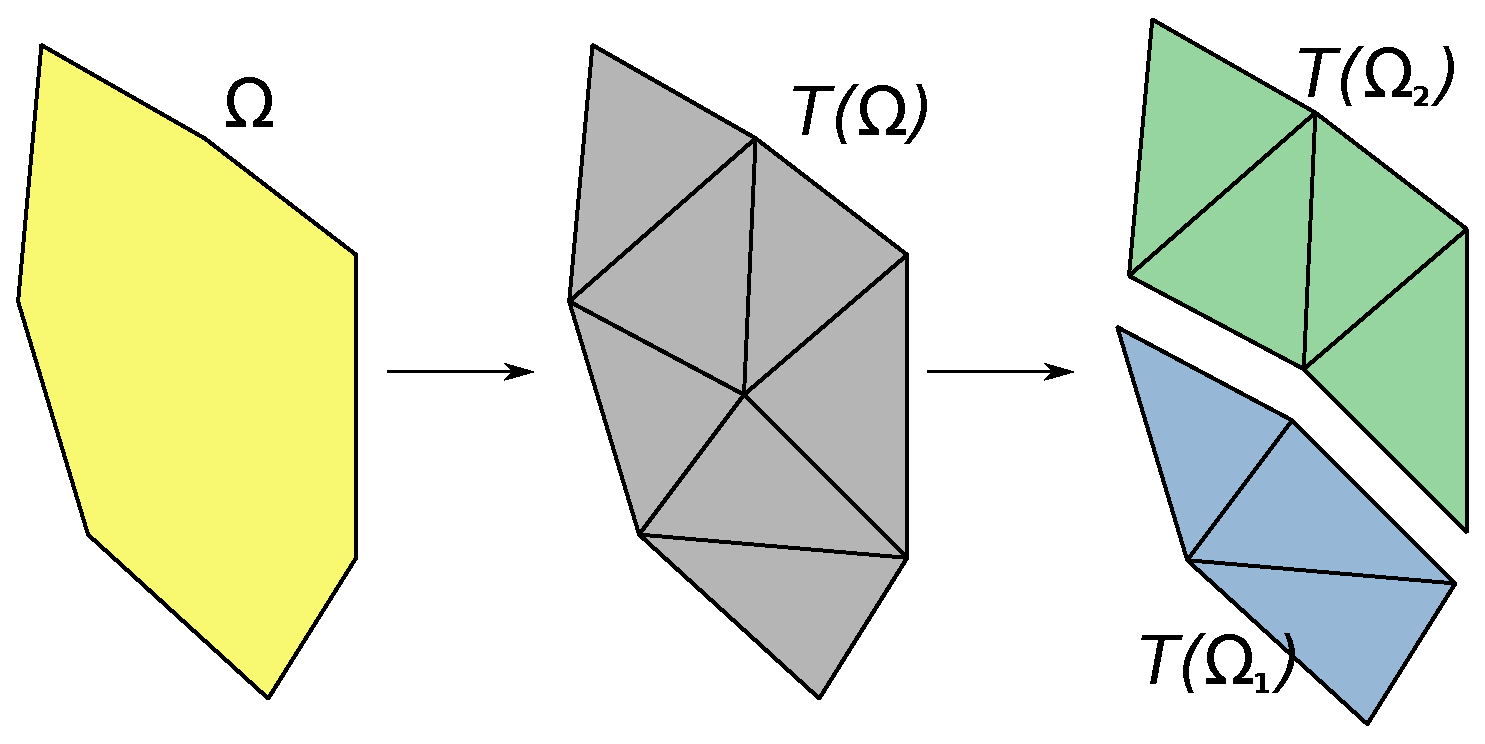
\includegraphics[width=.6\linewidth]{EPS/dd}
  \end{center}

\end{frame}

\subsubsection{Nonoverlapping Domain Decomposition}
\begin{frame}
  \frametitle<presentation>{Nonoverlapping Domain Decomposition}

  \begin{columns}
    \begin{column}{0.6\linewidth}
      % In overlapping domain decomposition methods, the subdomains
      % overlap by more than the interface. Overlapping domain
      % decomposition methods
      % include the Schwarz alternating method and the additive
      % Schwarz
      % method. Many domain decomposition methods can be written and
      % analyzed as a special case of the abstract additive Schwarz
      % method.
    
      \begin{itemize}
      \item Given a domain $\Omega\subseteq\mathbb{R}^d$
        % and a triangulation $T(\Omega) = \{E\}$
        % \item partition the cells $E$ such that there is exactly one
        %   processor with $E \in T(\Omega_i)$
      \item partition $\Omega$ into \emph{non-overlapping}
        sub-domains:
        \[
        \Omega_i\colon\quad \bigcup_{i=1}^p \overline{\Omega_i} = \overline{\Omega}, \quad
        \Omega_i\cap\Omega_j=\emptyset \;\forall i\ne j.
        \]
      \end{itemize}
    \end{column}
    \begin{column}{0.4\linewidth}
      \begin{onlyenv}<presentation>
        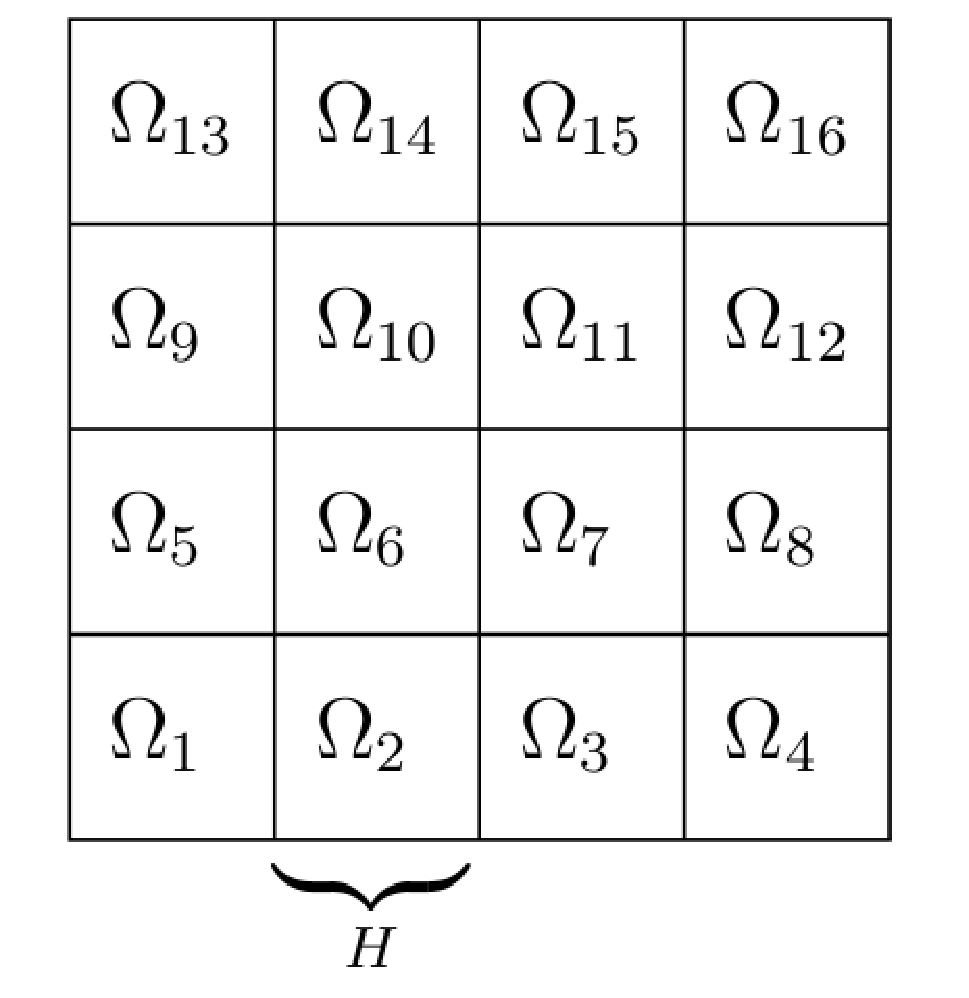
\includegraphics[width=0.6\linewidth]{EPS/konstr_n_uberl_str}
        \vskip5mm
        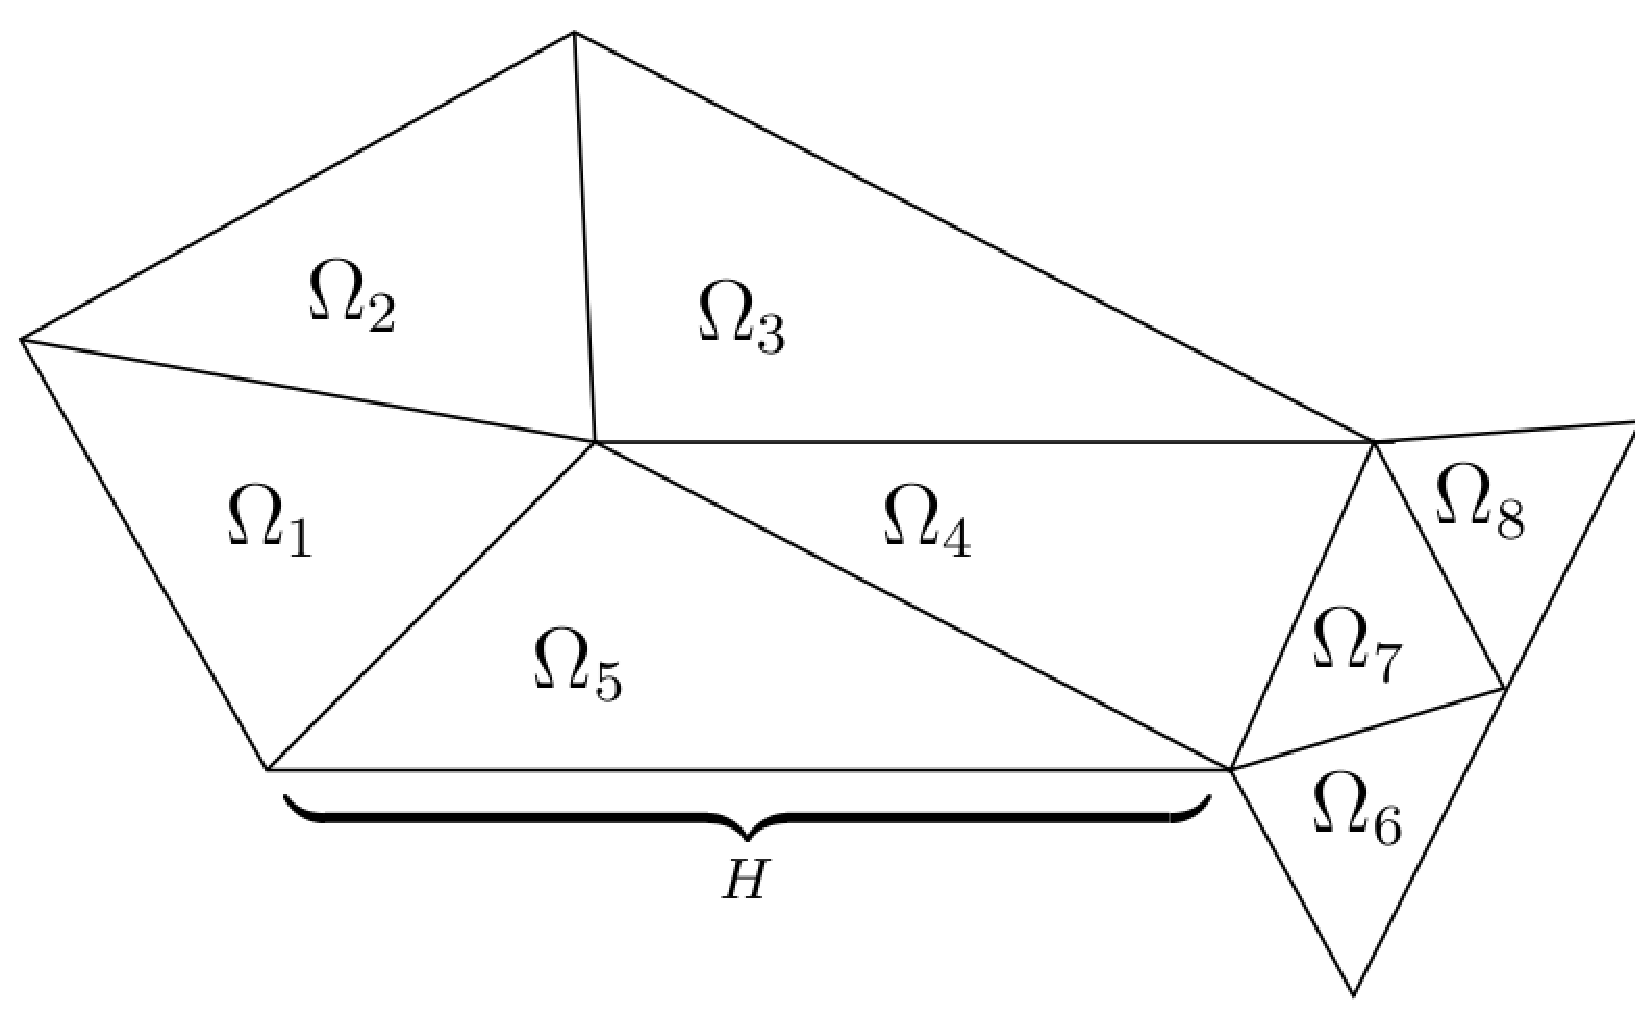
\includegraphics[width=0.9\linewidth]{EPS/konstr_n_uberl_unstr}
      \end{onlyenv}
      \begin{onlyenv}<article>
        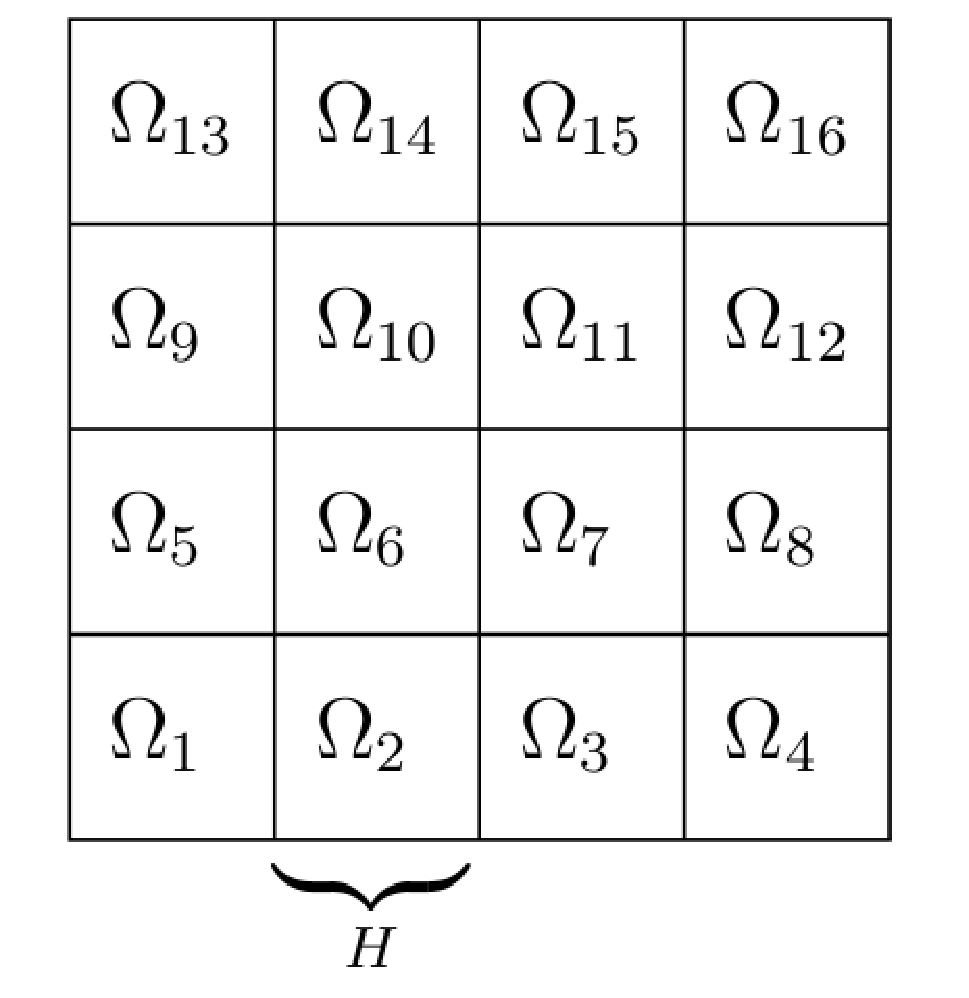
\includegraphics[width=0.25\linewidth]{EPS/konstr_n_uberl_str}
        \vskip5mm
        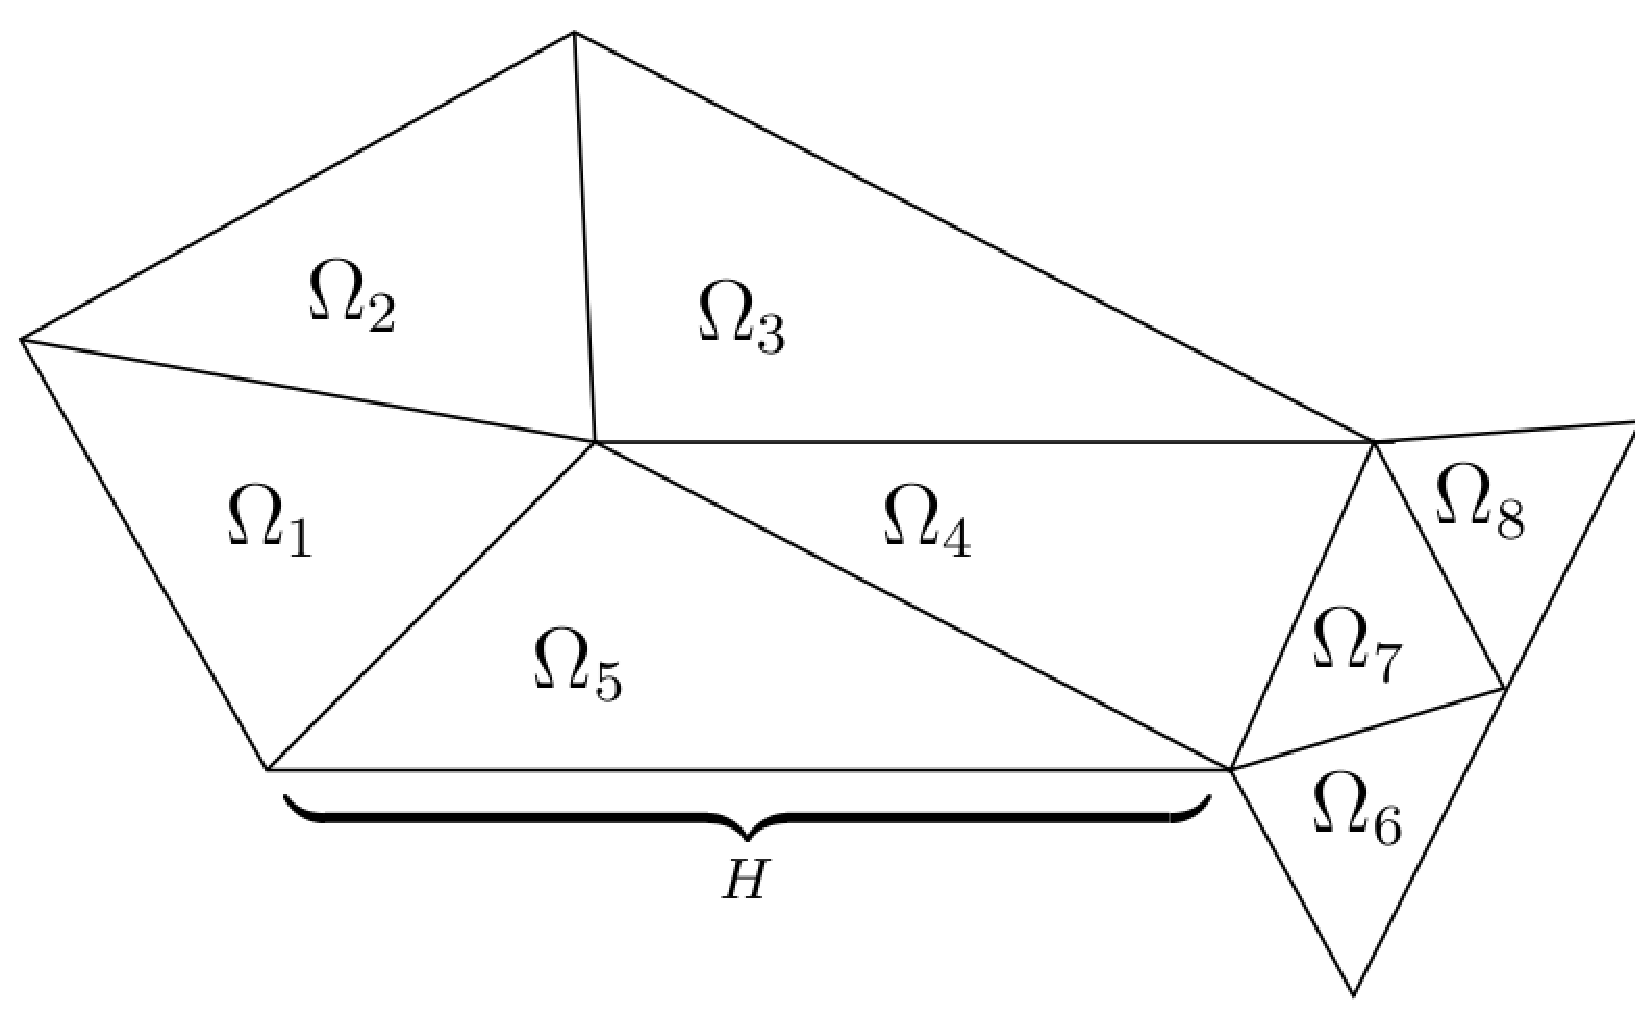
\includegraphics[width=0.36\linewidth]{EPS/konstr_n_uberl_unstr}
      \end{onlyenv}
    \end{column}
  \end{columns}
\end{frame}

\subsubsection{Overlapping Domain Decomposition}
\begin{frame}
  \frametitle<presentation>{Overlapping Domain Decomposition}

  \begin{columns}
    \begin{column}{0.6\linewidth}
      % In overlapping domain decomposition methods, the subdomains
      % overlap by more than the interface. Overlapping domain
      % decomposition methods
      % include the Schwarz alternating method and the additive
      % Schwarz
      % method. Many domain decomposition methods can be written and
      % analyzed as a special case of the abstract additive Schwarz
      % method.
    
      \begin{itemize}
      \item Extend each $\Omega_i$ by an overlap $\hat \Omega_i$ of width
        $\beta\cdot H$:
        \[
        \hat \Omega_i = \left\{ x\in\Omega \mid \mathsf{dist}(x,\Omega_i) < \beta\cdot H \right\}
        \]
      \end{itemize}
    \end{column}
    \begin{column}{0.4\linewidth}
      \begin{onlyenv}<presentation>
        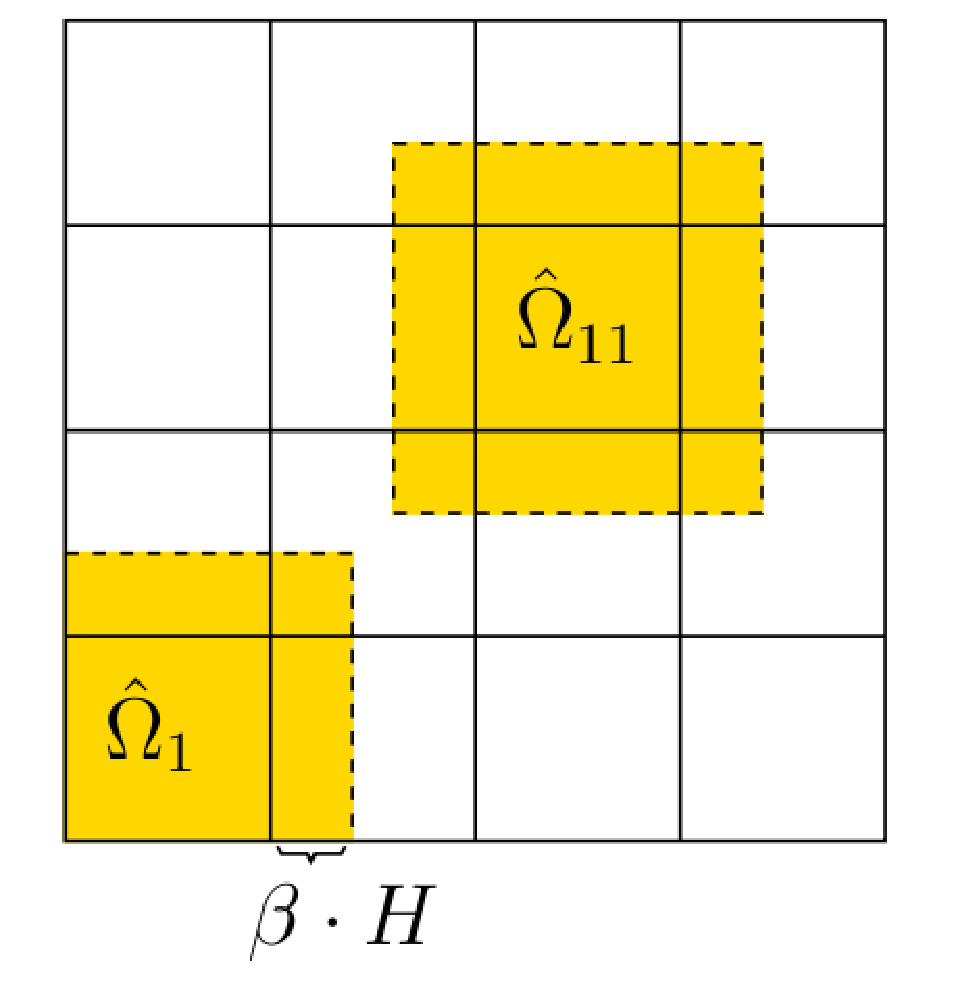
\includegraphics[width=0.6\linewidth]{EPS/konstr_uberl_str}
        \vskip5mm
        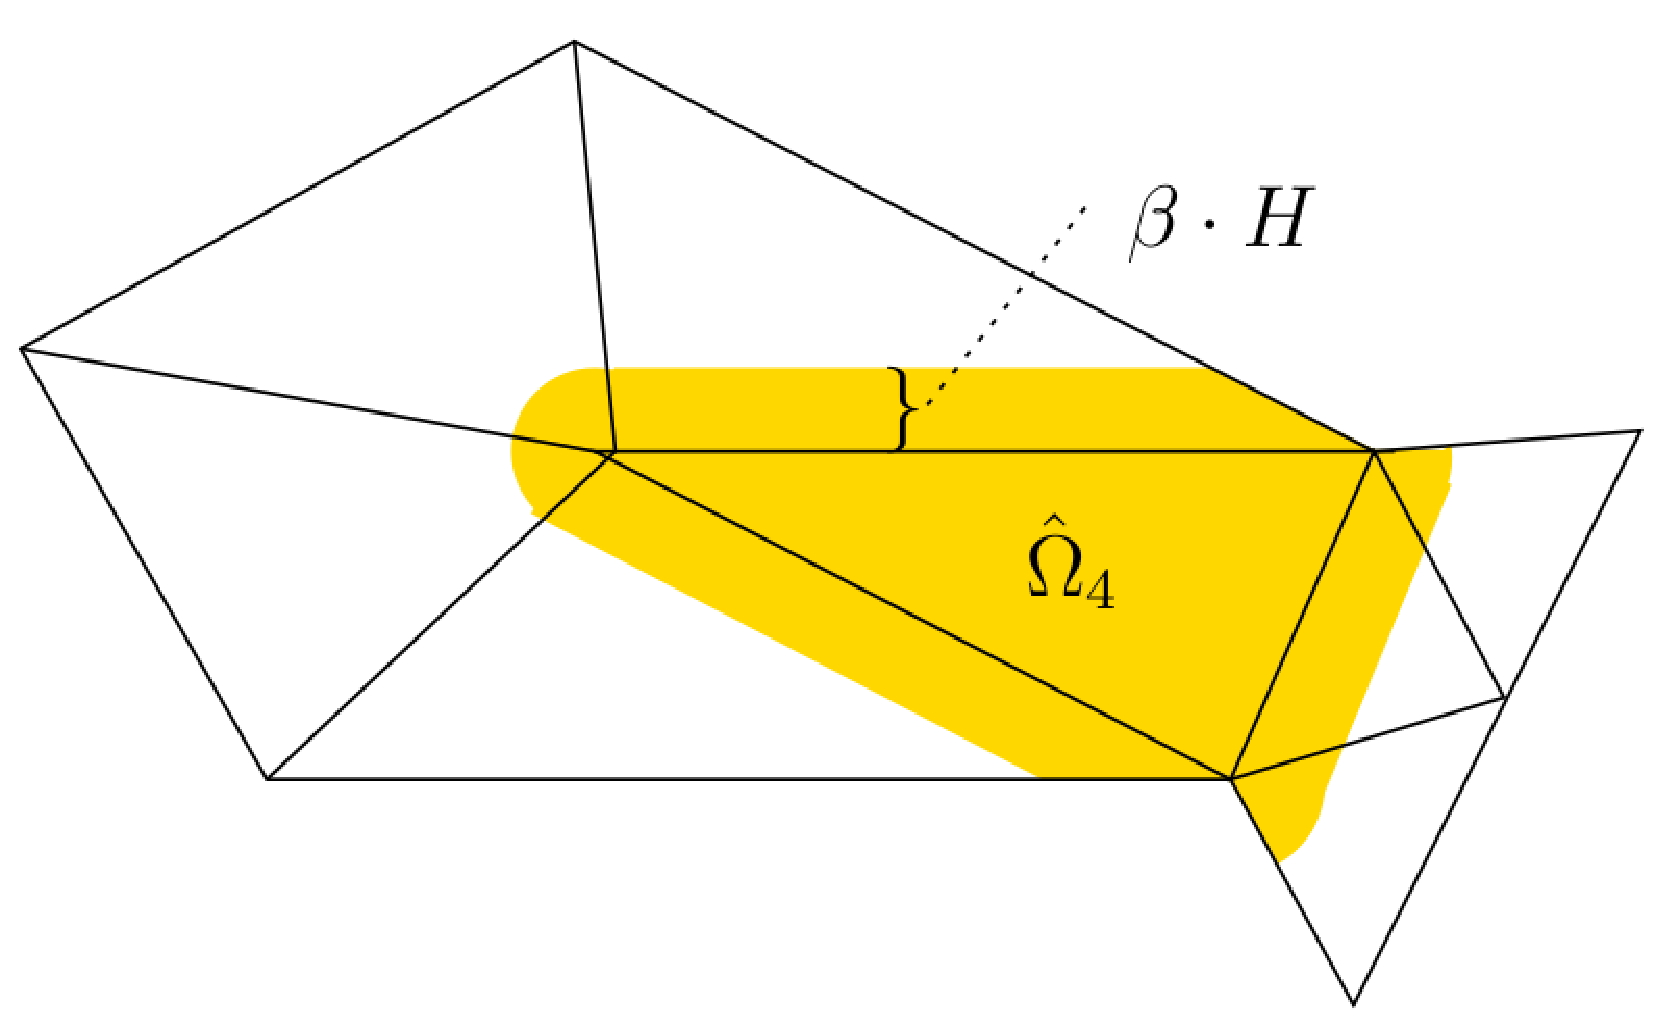
\includegraphics[width=0.9\linewidth]{EPS/konstr_uberl_unstr}
      \end{onlyenv}
      \begin{onlyenv}<article>
        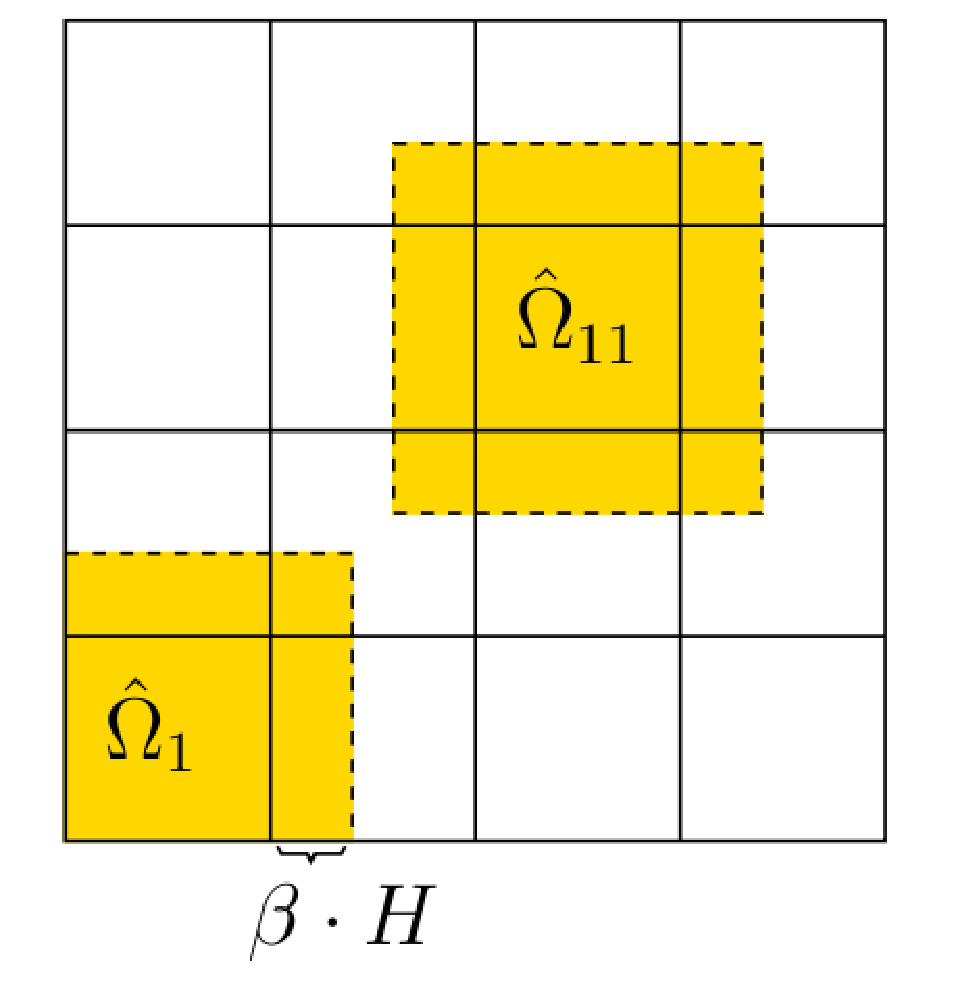
\includegraphics[width=.25\linewidth]{EPS/konstr_uberl_str}
        \vskip5mm
        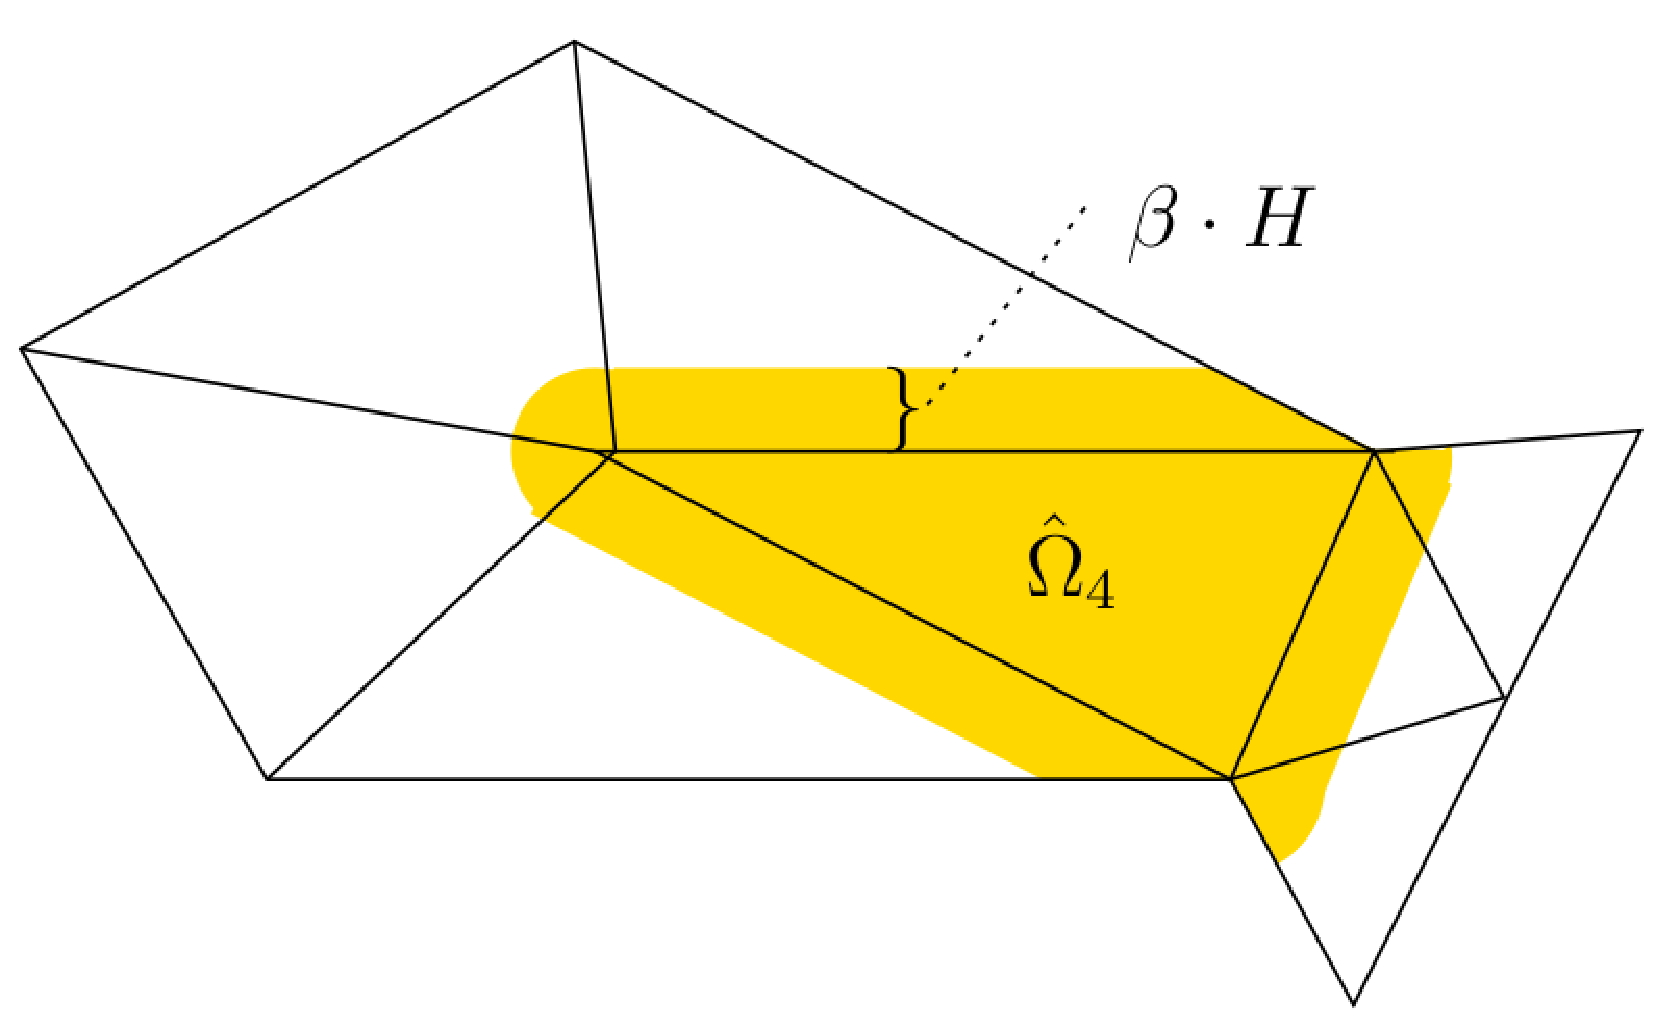
\includegraphics[width=.36\linewidth]{EPS/konstr_uberl_unstr}
      \end{onlyenv}
    \end{column}
  \end{columns}
\end{frame}

\subsection{Parallel Grids}
%-----------------------------------------------------------------------------

\subsubsection{Partition Types}
\begin{frame}[fragile]
\frametitle<presentation>{Partition Types}

\begin{itemize}
\item Each grid entity can be present on one or more processors.
\item Each entity on one processor has a partition type, which can be determined 
by the method\\
        \hspace*{1cm}\lstinline!entity.partitionType()!
\item The possible partition types are:\\
\end{itemize}
\begin{tabular}{ll}
  \em \bfseries interior 
  & Entity is owned by the process\\
  \em \bfseries overlap & Entity is owned by a different process, but a full copy exists\\
  \em \bfseries ghost
  & Entity is owned by a different process, but a partial copy\\
  & exists\\
  \em \bfseries border
  & Boundary of interior. (only exists for entities with \\
  & codimension$>$0)\\
  \em \bfseries front
  & Boundary of interior+overlap if not {\em \bfseries border} (only exists for\\
  & entities with codimension$>$0)
\end{tabular}
\end{frame}


\begin{frame}[fragile]
\frametitle{Partition Types Example}
\begin{columns}[c]
\begin{column}{0.7\textwidth}

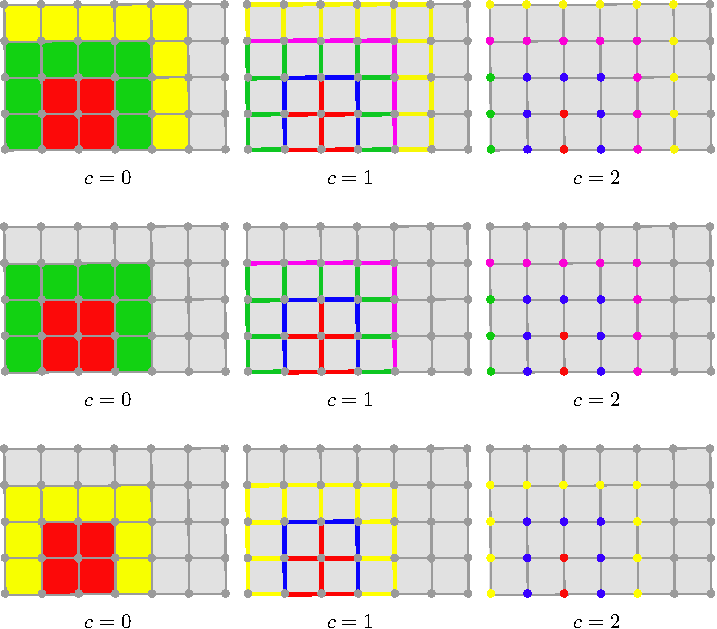
\includegraphics[width=\textwidth]{EPS/partitionsingle}
\end{column}
\begin{column}{0.3\textwidth}
\vskip0.5cm
\textbf{First row}: with overlap and ghosts\\
\textbf{Second row}: with overlap only\\
\textbf{Third row}: with ghosts only
\vskip5mm
\begin{center}
\begin{tabular}{|c|}
\hline\color{red} interior\\\hline
\color{green} overlap\\\hline
\color{yellow} ghost\\\hline
\color{blue} border\\\hline
\color{magenta} front\\\hline
\color{gray} not stored\\\hline
\end{tabular}
\end{center}
\end{column}
\end{columns}

\end{frame}

\subsubsection{Parallel Grids in Dune}

\begin{frame}
  \frametitle<presentation>{Parallel Grids in Dune}
  \begin{itemize}
  \item<1-> \lstinline[basicstyle=\normalfont\ttfamily]!YaspGrid!
      \begin{itemize}
      \item structured
      \item 2D/3D
      \item arbitrary overlap
      \end{itemize}
  \item<2-> \lstinline[basicstyle=\normalfont\ttfamily]!UGGrid!
      \begin{itemize}
      \item unstructured
      \item 2D/3D
      \item multi-element
      \item one layer of ghost cells
      \item (conforming) red-green refinement
      \item (non-free!)
      \end{itemize}
  \item<3-> \lstinline[basicstyle=\normalfont\ttfamily]!ALUGrid!
      \begin{itemize}
      \item unstructured
      \item 3D
      \item tetrahedral or hexahedral elements
      \item ghost cells
      \item (non-conforming) bisection refinement
      \end{itemize}
  \end{itemize}
\end{frame}

\subsubsection{Iterators in a parallel Grid}

\begin{frame}[fragile]
  \frametitle<presentation>{Iterators in a parallel Grid}
  \small
  Dune offers Iterators which only iterate over elements with certain partition types:\\
\begin{lstlisting}
Grid::template Codim<c>::template Partition<ptype>::Iterator it = gridView.template begin<c,ptype>();
\end{lstlisting}

\lstinline!ptype! is one of:
  \begin{center}
    \begin{tabular}{ll}
      \texttt{Interior\_Partition} & interior entities only\\
      \texttt{InteriorBorder\_Partition} & interior entities plus border (identical to \\
                                         & \texttt{Interior\_Partition} for entities of \\
                                         & codimension==0)\\
      \texttt{Overlap\_Partition} & overlap entities only\\
      \texttt{OverlapFront\_Partition} & overlap entities plus front (identical to \\
                                       & \texttt{Overlap\_Partition} for entities of \\
                                       & codimension==0)\\
      \texttt{Ghost\_Partition} & ghost entities only\\
      \texttt{All\_Partition} & all entities available to the process
    \end{tabular}
  \end{center}
%   \item<2>[\em Note:] \emph{The index set always contains indices for all
%     entities in the \lstinline!All_Partition!.}
%   \end{description}
\end{frame}

\subsubsection{Additional Remarks}

%-----------------------------------------------------------------------------
\begin{frame}
\frametitle<presentation>{Additional Remarks}
\begin{itemize}
\item On each intersection there exists a method \lstinline!neighbor()!. This method returns \lstinline!true! if there is a 
neighbor available on the same process.
\item The method \lstinline!boundary()! only returns \lstinline!true! at the domain boundary (even if the grid is periodic at this boundary) not at a process boundary.
\end{itemize}
\end{frame}

\subsection{Communicating Data with Dune}
\begin{frame}[fragile]
  \frametitle<presentation>{Communicating Data with Dune}

%% local index

  \begin{itemize}
  \item Data is associated with grid entities using an \texttt{IndexSet}.
  \item The index set provides indices for all entities stored on the process (i.e. the \texttt{All\_Partition})
  \item Data is stored locally.
  \item Algorithms may require data exchange e.g. for synchronization or the calculation of updates 
  \item Dune provides methods for the communication of data and methods for collective communication
  \end{itemize}

\end{frame}

\subsubsection{Communication API}
\begin{frame}[fragile]
  \frametitle<presentation>{Communication API}

  \texttt{GridView} provides a method for the communication between processes
    \begin{lstlisting}
template<class DHImp, class DataType>
void communicate ( CommDataHandleIF<DHImp, DataType> &datahandle, InterfaceType interface, CommunicationDirection dir ) const;
    \end{lstlisting}
where
    \begin{itemize}
    \item \lstinline!CommDataHandleIF!\\
      is a user defined class describing what data should be communicated. The class has to provide methods to read (gather) the data on the
      source process and write (scatter) the data on the target process.
    \end{itemize}
\end{frame}


\begin{frame}[fragile]
  \frametitle<presentation>{Communication API}
  \begin{onlyenv}<presentation>
  \texttt{GridView} provides a method for the communication between processes
    \begin{lstlisting}
template<class DHImp, class DataType>
void communicate ( CommDataHandleIF<DHImp, DataType> &datahandle, InterfaceType interface, CommunicationDirection dir ) const;
    \end{lstlisting}
where
    \end{onlyenv}
    \begin{itemize}
    \item \lstinline!InterfaceType!\\
    Determines the partition type of the entities to be sent and received. With \lstinline!InteriorBorder_InteriorBorder_Interface! only
border entities are sent. With \lstinline!All_All_Interface!,
    \lstinline!InteriorBorder_All_Interface! and
    \lstinline!Overlap_All_Interface! all entities, only interior and border entities or only overlap entities are sent. Only processes with common
data communicate and only the entities present on both processes are included in the communication.
    \item \lstinline!CommunicationDirection!
      The direction of the communication can be changed with either \lstinline!ForwardDirection! or
      \lstinline!BackwardDirection!
    \end{itemize}
\end{frame}



\subsubsection{Collective Communication}

\begin{frame}[fragile]
  \frametitle<presentation>{CollectiveCommunication}
  \structure{Problem:}
  \begin{itemize}
  \item parallel computations require global communication (e.g. sum(defect) or $\min(\Delta t)$ 
        and synchronization (e.g. a barrier needed for a timing)
  \item Dune grids provide a collective communicator method:
    \lstinline!  const CollectiveCommunication & comm () const;!
  \end{itemize}
  
  \lstinline[basicstyle=\normalfont\ttfamily]!Dune::Grid::CollectiveCommunication! provides:
 \begin{center}
    \scriptsize
    \begin{tabular}{l|l}
      \hline
      Method name & Description\\\hline
      \lstinline!rank! & obtain number (rank) of this process\\
      \lstinline!size! & obtain number of processes \\
      \lstinline!barrier! & wait till all process arrived\\
      \lstinline!min! & global min of local values\\
      \lstinline!max! & global max of local values\\
      \lstinline!sum! & global sum of local values\\
      \lstinline!broadcast! & broadcast from one process to all other processes\\
      \dots\\
      \hline
    \end{tabular}    
 \end{center}
  
\end{frame}

\subsubsection{Load-Balancing and Adaptation}
\begin{frame}[fragile]
  \frametitle<presentation>{Load-Balancing}
  \structure{Problem:}
  \begin{itemize}
  \item parallelization only scales well if all processes have the
    same work load\\
    $\Rightarrow$ well balanced grids
  \item adaptation leads to unbalanced work load
  \item only 3D ALUGrid provides working load balance methods to re-balance the work load
  \begin{description}[123]
  \item[\tt loadBalance(DataHandle \&data)]:\\
    re-balances a parallel grid, optionally send also user data
  \item[\tt DataHandle]:\\
    works like the data handle for the communicate methods
  \end{description}
   \item with UGGrid you can initialize a coarse grid and then call \lstinline!loadBalance! before starting the
         computation.
  \end{itemize}
\end{frame}

\begin{frame}[fragile]
  \frametitle{Grid-Distribution with YaspGrid}
With YaspGrid you can determine how the grid is partitioned (as it is a structured grid
adaptive grid refinement and load-balancing are not possible) by writing a class derived from
\lstinline!Dune::YLoadBalance<dim>!

\begin{lstlisting}
template<int dim>
class YaspPartition : public Dune::YLoadBalance<dim>
{
  private:
    const unsigned &numProc;  // number of processes
  public:
    YaspPartition( const unsigned &numProc_ ) : numProc( numProc_ )
    {}

    typedef Dune::FieldVector<int, dim>  iTupel;
    void loadbalance (const iTupel& size, int P, iTupel& dims) const
    {
      dims = 1;
      dims[1]= numProc;
    }
};
\end{lstlisting}
\end{frame}

\begin{frame}[fragile]
  \frametitle<presentation>{Grid-Distribution with YaspGrid}
Now you can pass the object to the constructor during grid creation
\begin{lstlisting}
Dune::FieldVector<int,2> n(10), overlap(1);
Dune::FieldVector<double,2> upper(1.0);
Dune::FieldVector<bool,dim> periodic(false);
YaspGrid<2> grid(upper, n, periodic, 0);
YaspPartition<dim> yp(mpiHelper.size());
GRID grid(mpiHelper.getCommunicator(), upper, n, periodic, overlap, &yp );
\end{lstlisting}
\end{frame}

\subsection{Parallel PDELab}

\begin{frame}
  \frametitle<presentation>{Parallel PDELab}
Parallel computing in PDELab is very easy. 
  \begin{itemize}
  \item Go parallel by choosing
    \begin{enumerate}
    \item a suitable parallel grid,
    \item the correct constraints for the discretization of
      the PDE (either \lstinline!OverlappingConformingDirichletConstraints! or \lstinline!NonoverlappingConformingDirichletConstraints!) , and
    \item a suitable and matching parallel solver backend of the
      PDELab backend.
    \end{enumerate}
  \end{itemize}
\end{frame}

\subsubsection{Parallel Solver Backends}
\begin{frame}
  \frametitle<presentation>{Parallel Solver Backends}

\begin{itemize}
\item ISTL solvers need to be provided a \lstinline!Preconditioner! (like Jacobi, SSOR or ILU), a 
\lstinline!LinearOperator! (providing a matrix-vector product) and
a \lstinline!ScalarProduct!. These versions of these components have to fit together.
\item Parallel solver backends make sure that the correct implementations of 
\lstinline!Preconditioner!, \lstinline!LinearOperator! and \lstinline!ScalarProduct!
are choosen matching the type of domain decomposition.
\item Different solver backends are provided for overlapping and nonoverlapping domain
decomposition.
\item The solver backends can be found in the headers \lstinline!dune/pdelab/backend/istlsolverbackend.hh!,
\lstinline!dune/pdelab/backend/ovlpistlsolverbackend.hh! and
\lstinline!dune/pdelab/backend/novlpistlsolverbackend.hh!.
\end{itemize}

\only<2>{
\alert{Please make sure that you always choose a matching solver for your type
of domain decomposition!!!}}
\end{frame}

\begin{frame}
  \frametitle<presentation>{Building Blocks for Parallel Solvers}
  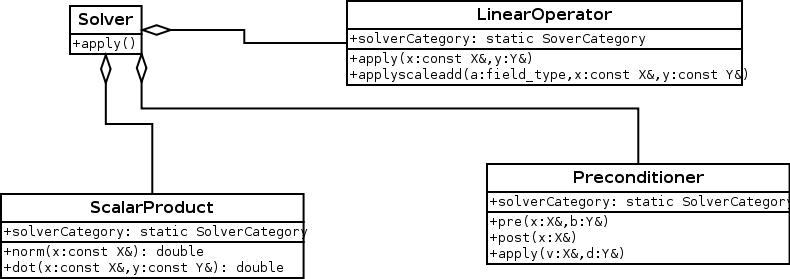
\includegraphics[width=\textwidth]{EPS/istlsolver}
\end{frame}

%-----------------------------------------------------------------------------

\begin{frame}
\frametitle{Parallel Preconditioners}
\begin{itemize}
\item To run in parallel Conjugate Gradients (CG) and BiCGStab solvers have to be able to compute parallel matrix vector
products and scalar products.
\item As parallel preconditioners to the CG and BiCGStab solvers additive Schwarz methods can be used:
\begin{itemize}
\item In this schemes the local subproblem on each processor is solved
where the values of the last iteration are used as Dirichlet constraints at the process boundary. 
\item Different solvers can be choosen for the local problems (e.g. a direct solver like SuperLU or some steps of an 
iterative solver like SSOR).
\item In an overlapping decomposition corrections are computed for the overlap at more than one process. The sum of the corrections multiplied with a relaxation 
coefficient is applied. 
\item With an overlapping Schwarz method the convergence is better the larger the overlap.
\end{itemize}
\item For overlapping domain decomposition there exists also an algebraic multigrid preconditioner.
\end{itemize}
\end{frame}


\begin{frame}
  \frametitle{Parallel Solver Backends for Overlapping DD}
The linear solvers in this table are preconditioned with an overlapping domain decomposition
using the respective smoother or with a parallel algebraic multigrid scheme with an SSOR smoother (AMG).
\begin{center}
\begin{tabular}{|l|l|l|}\hline
solver backend & smoother & linear solver\\\hline
\lstinline!ISTLBackend_OVLP_CG_SSORk<GFS,C>! & SSOR & CG\\\hline
\lstinline!ISTLBackend_OVLP_CG_SuperLU<GFS,C>! & SuperLU & CG\\\hline
\lstinline!ISTLBackend_CG_AMG_SSOR<GFS>! & AMG & CG\\\hline
\lstinline!ISTLBackend_OVLP_BCGS_SSORk<GFS,C>! & SSOR & BiCGStab\\\hline
\lstinline!ISTLBackend_OVLP_BCGS_SuperLU<GFS,C>! & SuperLU & BiCGStab\\\hline
\lstinline!ISTLBackend_BCGS_AMG_SSOR<GFS>! & AMG & BiCGStab\\\hline
\end{tabular}
\end{center}
\lstinline!ISTLBackend_OVLP_ExplicitDiagonal<GFS>! is a solver for explicit 
time-steppers with (block-)diagonal mass matrix.

The template parameter \lstinline!GFS! is the grid function space, \lstinline!C! is the type of the 
constraints container (usually \lstinline!OverlappingConformingDirichletConstraints!).
\end{frame}

\begin{frame}[fragile]
  \frametitle{Overlapping Example}
  \begin{lstlisting}[basicstyle=\small]
// 1. Create an overlapping grid
Dune::FieldVector<double,2> L(1.0);
Dune::FieldVector<int,2> N(16);
Dune::FieldVector<bool,2> periodic(false);
int overlap=2; 
Dune::YaspGrid<2> grid(helper.getCommunicator(),L,N,periodic,overlap);
typedef Dune::YaspGrid<2>::LeafGridView GV;
const GV& gv=grid.leafView();

// 2. Create correctly constrained grid function space
typedef Dune::PDELab::Q1LocalFiniteElementMap<Coord,Real,dim> FEM;
FEM fem;
typedef Dune::PDELab::OverlappingConformingDirichletConstraints CON;
typedef Dune::PDELab::ISTLVectorBackend<1> VBE;
typedef Dune::PDELab::GridFunctionSpace<GV,FEM,CON,VBE,
Dune::PDELab::SimpleGridFunctionStaticSize> GFS;
GFS gfs(gv,fem);

//  define problem parameters
typedef ConvectionDiffusionProblem<GV,Real> Param;
Param param;
typedef Dune::PDELab::BoundaryConditionType_CD<Param> B;
B b(gv,param);
typedef Dune::PDELab::DirichletBoundaryCondition_CD<Param> G;
G g(gv,param);
\end{lstlisting}  
\end{frame}
\begin{frame}[fragile]
\frametitle<presentation>{Overlapping Example Continued}
  \begin{lstlisting}[basicstyle=\small]

//  Compute constrained space
typedef typename GFS::template ConstraintsContainer<Real>::Type C;
C cg;
Dune::PDELab::constraints(b,gfs,cg);
//  Compute affine shift
typedef typename GFS::template VectorContainer<Real>::Type V;
V x(gfs,0.0);
Dune::PDELab::interpolate(g,gfs,x);
Dune::PDELab::set_nonconstrained_dofs(cg,0.0,x);
// Make grid operator space
typedef Dune::PDELab::ConvectionDiffusion<Param> LOP; 
LOP lop(param,2);
typedef Dune::PDELab::ISTLBCRSMatrixBackend<1,1> MBE;
typedef Dune::PDELab::GridOperatorSpace<GFS,GFS,LOP,C,C,MBE> GOS;
GOS gos(gfs,cg,gfs,cg,lop);

// 3. Choose a linear solver 
typedef Dune::PDELab::ISTLBackend_OVLP_BCGS_SuperLU<GFS,C> LS;
LS ls(gfs,cg,5000,2);
...
\end{lstlisting}
\end{frame}

\begin{frame}
  \frametitle{Parallel Solver Backends for Nonoverlapping DD}
The linear solvers in this table are preconditioned with a nonoverlapping domain decomposition
using the respective smoother.
\begin{center}
\begin{tabular}{|l|l|l|}\hline
solver backend & smoother & linear solver\\\hline
\lstinline!ISTLBackend_NOVLP_CG_NOPREC<GFS>! & -- & CG\\\hline
\lstinline!ISTLBackend_NOVLP_CG_Jacobi<GFS>! & Jacobi & CG\\\hline
\lstinline!ISTLBackend_NOVLP_CG_SSORk<GOS,Scalar>! & SSOR & CG\\\hline
\lstinline!ISTLBackend_NOVLP_BCGS_NOPREC<GFS>! & -- & BiCGStab\\\hline
\lstinline!ISTLBackend_NOVLP_BCGS_SSORk<GOS,Scalar>! & SSOR & BiCGStab\\\hline
\end{tabular}
\end{center}
\lstinline!ISTLBackend_NOVLP_ExplicitDiagonal! is a solver for explicit 
time-steppers with (block-)diagonal mass matrix.

The template parameter \lstinline!GFS! is the grid function space, \lstinline!GOS! is the grid operator space
and \lstinline!Scalar! the type of a scalar value in the matrix.
\end{frame}

\begin{frame}[fragile]
  \frametitle{Nonoverlapping example}
  \begin{lstlisting}[basicstyle=\small]
// 1. Create an non-overlapping grid
Dune::FieldVector<double,2> L(1.0);
Dune::FieldVector<int,2> N(16);
Dune::FieldVector<bool,2> periodic(false);
int overlap=0; // needs overlap 0 because overlap elements are not assembled
Dune::YaspGrid<2> grid(helper.getCommunicator(),L,N,periodic,overlap);
typedef Dune::YaspGrid<2>::LeafGridView GV;
const GV& gv=grid.leafView();

// 2. Create correctly constrained grid function space
typedef Dune::PDELab::Q1LocalFiniteElementMap<Coord,Real,dim> FEM;
FEM fem;
typedef Dune::PDELab::NonoverlappingConformingDirichletConstraints CON;
CON con;
typedef Dune::PDELab::ISTLVectorBackend<1> VBE;
typedef Dune::PDELab::GridFunctionSpace<GV,FEM,CON,VBE,
Dune::PDELab::SimpleGridFunctionStaticSize> GFS;
GFS gfs(gv,fem,con);
con.compute_ghosts(gfs); // con stores indices of ghost dofs
typedef ConvectionDiffusionProblem<GV,Real> Param;
Param param;
typedef Dune::PDELab::BoundaryConditionType_CD<Param> B;
B b(gv,param);
typedef Dune::PDELab::DirichletBoundaryCondition_CD<Param> G;
G g(gv,param);
\end{lstlisting}
\end{frame}
\begin{frame}[fragile]
\frametitle<presentation>{Nonoverlapping Example Continued}
  \begin{lstlisting}[basicstyle=\small]
// Compute constrained space
typedef typename GFS::template ConstraintsContainer<Real>::Type C;
C cg;
Dune::PDELab::constraints(b,gfs,cg);

// Compute affine shift
typedef typename GFS::template VectorContainer<Real>::Type V;
V x(gfs,0.0);
Dune::PDELab::interpolate(g,gfs,x);
Dune::PDELab::set_nonconstrained_dofs(cg,0.0,x);

// Make grid operator space
typedef Dune::PDELab::ConvectionDiffusion<Param> LOP; 
LOP lop(param,2);
typedef Dune::PDELab::ISTLBCRSMatrixBackend<1,1> MBE;
typedef Dune::PDELab::GridOperatorSpace<GFS,GFS,LOP,C,C,MBE,true> GOS;
GOS gos(gfs,cg,gfs,cg,lop);

// 3. Choose a linear solver 
typedef Dune::PDELab::ISTLBackend_NOVLP_BCGS_NOPREC<GFS> LS;
LS ls(gfs,5000,1);
...
\end{lstlisting}
  
\end{frame}

